%!TEX ROOT=../ctutest.tex

\chapter{State of the Art}
%--- FIG: UTF forms

This chapter will first describe the originally popular models for NLP such as BERT and the recent paradigm shift from \textit{pre-train+fine-tune} transfer learning framework popular since the original~\cite{devlin2019bert} paper to the currently booming LLMs which often outperform the smaller models even without the fine-tuning step~\cite{gpt4,llama,vicuna}. We will then take a look at the performance optimization methods that enable training multi-billion parameter pre-trained models on a set of task-specific data on a single GPU and their potential for our research. 

\label{chap:sota}
\section{Pre-train + Fine-tune}
\label{sec:pretrain}
Surprisingly well performing paradigm for small data, vague tasks
\subsection{BERT and derivatives}
Simple training task, scalable architecture, potential to evolve into something grand, czert, herbert, slovakbert

\dots Which currently arrives in form of:

\section{Large Language Models}
\label{sec:llms}
\subsection{GPT-3.5 and GPT-4}
\label{sec:gpt}
Obscure, paid~\cite{gpt3,gpt4}

\subsection{LLaMA-2 and derivatives}
\label{sec:llama}
Open-source, freely usable.
Often poor czech coverage 
Quantizace, 4b, 8b, zlomek parametrů\cite{openassistant}

\subsection{LoRA and other optimization}
To be able to fine-tune multi-billion-parameter models such as \textsf{LLaMA-2}~\cite{llama2} on a single TPU, multiple adjustments must be made to reduce the computational complexity.~\cite{peft}
\cite{lora}

\section{Fact checking approaches}
\subsection{FEVER and followups}
Yields interesting benchmark with statistically quantifiable model succes, oversimplificates the problem, as it uses Wikipedia for a trusted knowledge base and only reasons based on a data from a fixed period of time, focusing on \"{atomic} claims that do not match the complexity of real-world factoids.
\subsection{Open-domain fact-checking}
This paper with bing for example uses the whole internet, but is that really what we want? Like, every lie can be backed with an internet -- at the end of the day you do need to draw the line of what to trust somewhere, which directly conflicts this design.


\begin{figure}
    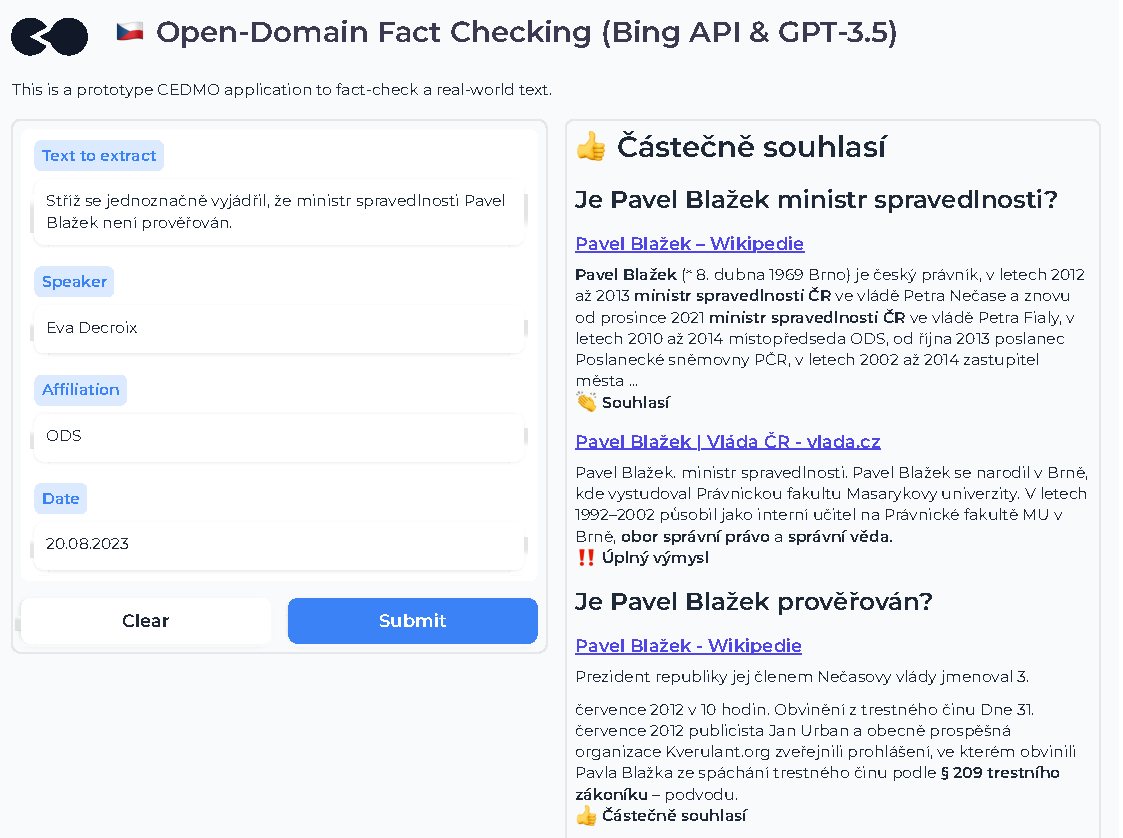
\includegraphics[width=14cm]{fig/bing.pdf}
    \caption{Proof-of-concept Czech fact-checking based on live-internet search (Bing API) and LLM prompting, based on the proposals of~\cite{bing} in Czech, using a real-world claim that was fact-checked by \href{https://demagog.cz/vyrok/22849}{\url{demagog.cz}} in June 2023}
    \label{fig:bing}
\end{figure}


\section{Claim generation}
\begin{itemize}
    \item Approches such as QACG exploit Question Answering
    \item The task of extreme summarization (XSum) focuses on summarizing a long body of text into a single sentence, focusing on its most relevant aspects and facts
    \item CLEF-CheckThat postulates the task of classifying \textit{Checkworthiness} of different parts of a long texts, such as a political debate
\end{itemize}

\section{NLP Generative task benchmarking}
\subsection{BERTScore}
\subsection{AlignScore}